\chapter{Theory of Beam Dynamics Relevant to the Large Hadron Collider}

\label{Chapter:Theory} % For referencing the chapter elsewhere, use \cref{Chapter:Theory}

%----------------------------------------------------------------------------------------

The design, operation, performance, and safety of a particle accelerator depend on the study of beam dynamics, a field of accelerator science.
This section provides an overview of the beam dynamics theories relevant to the material in this thesis, and more specifically beam optics.
Most of the material in this section can be found in the literature such as \cite{BOOK:Wilson:Introcution_Particle_Accelerators, BOOK:Lee:Accelerator_physics, BOOK:Wiedemann:Particle_Accelerator_Physics, BOOK:Minty:Measurements_Control_Charged_Particle_Beams,BOOK:Wolski:Beam_dynamics,BOOK:Chao:Handbook_Accelerator_Physics_Engineering, BOOK:Chao:Collective_instabilities}.
When not in these works, explicit references to content are given.
\todo{The chapter starts out with a description of linear dynamics, then moves on to aspects of non-linear dynamics, and ends with a discussion of luminosity}.

%----------------------------------------------------------------------------------------

\section{Linear Beam Dynamics}

The linear dynamics of an accelerator are, mainly, the endeavor to bend and focus particle beams to confine them within the machine's aperture.

\subsection{Transport and Guiding of Charged Particles}

To force the beam's particles into a closed trajectory, they are subjected to magnetic fields that deflect their trajectories.
The force exerted onto the beam is the Lorentz force \(F_{L}\), given by the equation:

\begin{equation}
    \vec{F_L} = \dfrac{d\vec{p}}{dt} = q (\vec{E} + \vec{v} \times \vec{B}) \text{ ,}
    \label{equation:lorentz_force}
\end{equation}
where \(p\) is the particle momentum, \(q\) the particle charge, \(\vec{E}\) the electric field, \(\vec{v}\) the particle velocity and \(\vec{B}\) the magnetic field.
In most accelerators, including the LHC, the particles' speed is close to the celerity of light \(c\) and the force from the magnetic field is significantly stronger than that produced by the electric field for realistic values of \(\vec{E}\) and \(\vec{B}\).
As a result, in high energy particle accelerators magnetic fields are typically used to guide particles.
The guiding magnetic field can be expanded into a series of multipolar fields, for instance here in the horizontal plane:
% ---------- Equation ----------
\begin{align}
    B_{y} = 
    \tikz[baseline]{
        \node[draw=red,rounded corners,anchor=base] (m1)
        {$\displaystyle B_{y0}$};
        \node[below of=m1] (l1) {dipole};
        \draw[-,red] (l1) -- (m1);
    }
    +
    \tikz[baseline]{
        \node[draw=red,rounded corners,anchor=base] (m2)
        {$\displaystyle \frac{dB_{y}}{dx} x$};
        \node[below of=m2] (l2) {quadrupole};
        \draw[-,red] (l2) -- (m2);
    }
    +
    \tikz[baseline]{
        \node[draw=red,rounded corners,anchor=base] (m3)
        {$\displaystyle \frac{1}{2!} \frac{d^2B_{y}}{dx^2} x^2$};
        \node[below of=m3] (l2) {sextupole};
        \draw[-,red] (l2) -- (m3);
    }
    +
    \tikz[baseline]{
        \node[draw=red,rounded corners,anchor=base] (m4)
        {$\displaystyle \frac{1}{3!} \frac{d^3B_{y}}{dx^3} x^3$};
        \node[below of=m4] (l2) {octupole};
        \draw[-,red] (l2) -- (m4);
    }
    + \ldots
    \label{equation:magnetic_field_expansion}
\end{align}

Bending forces are supplied by dipole magnets with a magnetic field perpendicular to the beam trajectory, while focusing is typically performed with the use of quadrupole magnets.
Higher orders belong to the nonlinear dynamics and will be discussed later on.
\Cref{figure:frenet_serret_system} illustrates the Frenet-Serret coordinate system traditionally used in linear beam dynamics.

\begin{figure}[!htb]
    \begin{center}
    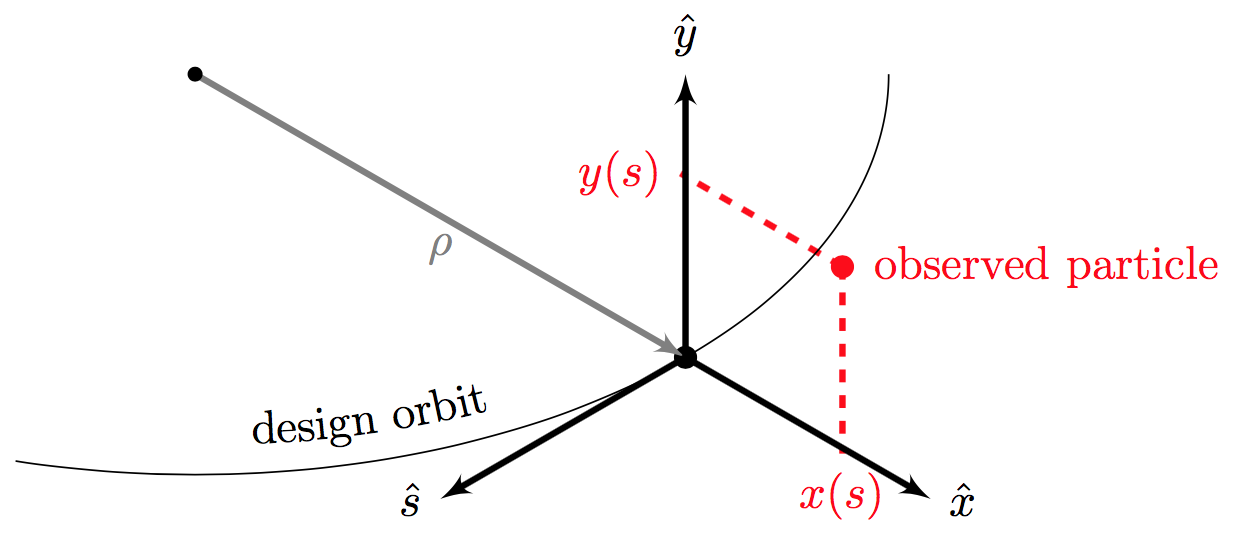
\includegraphics[width = 0.8\linewidth]{Figures/Chapter2/Frenet_Serret_Coordinate_System.png}
    \caption{The Frenet-Serret coordinate system used in accelerator physics. Here \(\hat{x}\), \(\hat{y}\), and \(\hat{s}\) form the right-handed orthogonal basis, while \(\rho\) is the local bending radius.}
    \label{figure:frenet_serret_system}
    \end{center}
\end{figure}

The coordinate system travels longitudinally with the particle, along a reference trajectory defined by an ideal, or \intro{synchronous}, particle.
The longitudinal curvilinear coordinate is \(s\), and denotes the position of the particle along the ideal orbit with respect to an arbitrary initial point at \(s = 0\).
One can define a local radius of curvature, \(\rho(s)\), which depends on the local magnetic field \(\vec{B}\) and varies along ring.
The transverse phase space is defined by \((x, x^{\prime}, y, y^{\prime})\), where \(x\) and \(y\) are a particle's coordinates in the transverse plane relative to the reference trajectory.
The \(x^{\prime}\) and \(y^{\prime}\) coordinates are \intro{divergent angles}, with the prime indicating differentiation with respect to \(s\).
\break

In the linear regime, magnetic dipoles define ideal orbit for a particle of \intro{reference momentum} \(p_0\).
This ideal orbit goes through the magnetic center of all elements in the machine to close back on itself after a revolution, and is called a \intro{closed orbit}.
In practice the real closed orbit will deviate from the ideal designed orbit due to various effects such as dipolar field errors.
Particles within the beam are distributed in amplitude and oscillate around the closed orbit, which corresponds to the path of a particle with zero amplitude within the beam, because of focusing forces. 
\break

Focusing forces are typically provided by magnetic quadrupoles: a quadrupolar field acting on a charged particle displaced from the closed orbit will provide a restoring (focusing) force proportional to the displacement in one transverse plane, while simultaneously providing a diverging (defocusing) force in the other. 
As a convention, a quadrupole focusing in the horizontal transverse plane and defocusing in the vertical is referred to as a \intro{focusing quadrupole}. 
Respectively, a quadrupole defocusing in the horizontal plane but focusing in the vertical is referred to as a \intro{defocusing quadrupole}.
A net focusing effect in both planes can be obtained with a setup of quadrupoles of alternating polarity in equal distance, a widely used configuration named the \(\mathrm{FODO}\) cell, a layout alternating quadrupoles in equal distance.
A schematic of a \(\mathrm{FODO}\) cell is shown in \cref{figure:fodo_cell_schematic}.

\begin{figure}[!htb]
    \begin{center}
    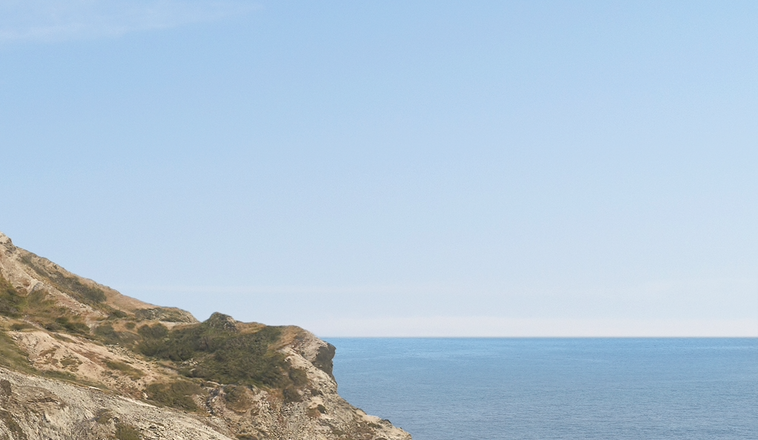
\includegraphics[width = 0.8\linewidth]{Figures/placeholder.png}
    \caption{\todo{Schematic of a \(\mathrm{FODO}\) cell. A focusing quadrupole is denoted with an F while a defocusing one is denoted with a D.}}
    \label{figure:fodo_cell_schematic}
    \end{center}
\end{figure}

For each magnet applying a field \(B\) one can define the \intro{magnetic rigidity}, which is an indication of the field’s ability to alter a particle’s course based on its charge \(q\) and momentum \(p\), as:

\begin{equation}
    B \rho = \frac{p}{q} \text{ .}
    \label{equation:magnetic_rigidity}
\end{equation}

\Cref{figure:dipole_quadrupole_fields} illustrates magnetic fields in an idealized dipole and quadrupole.

\begin{figure}[htp]
    \centering
    \subfloat[.7\linewidth][Ideal dipole.]{
        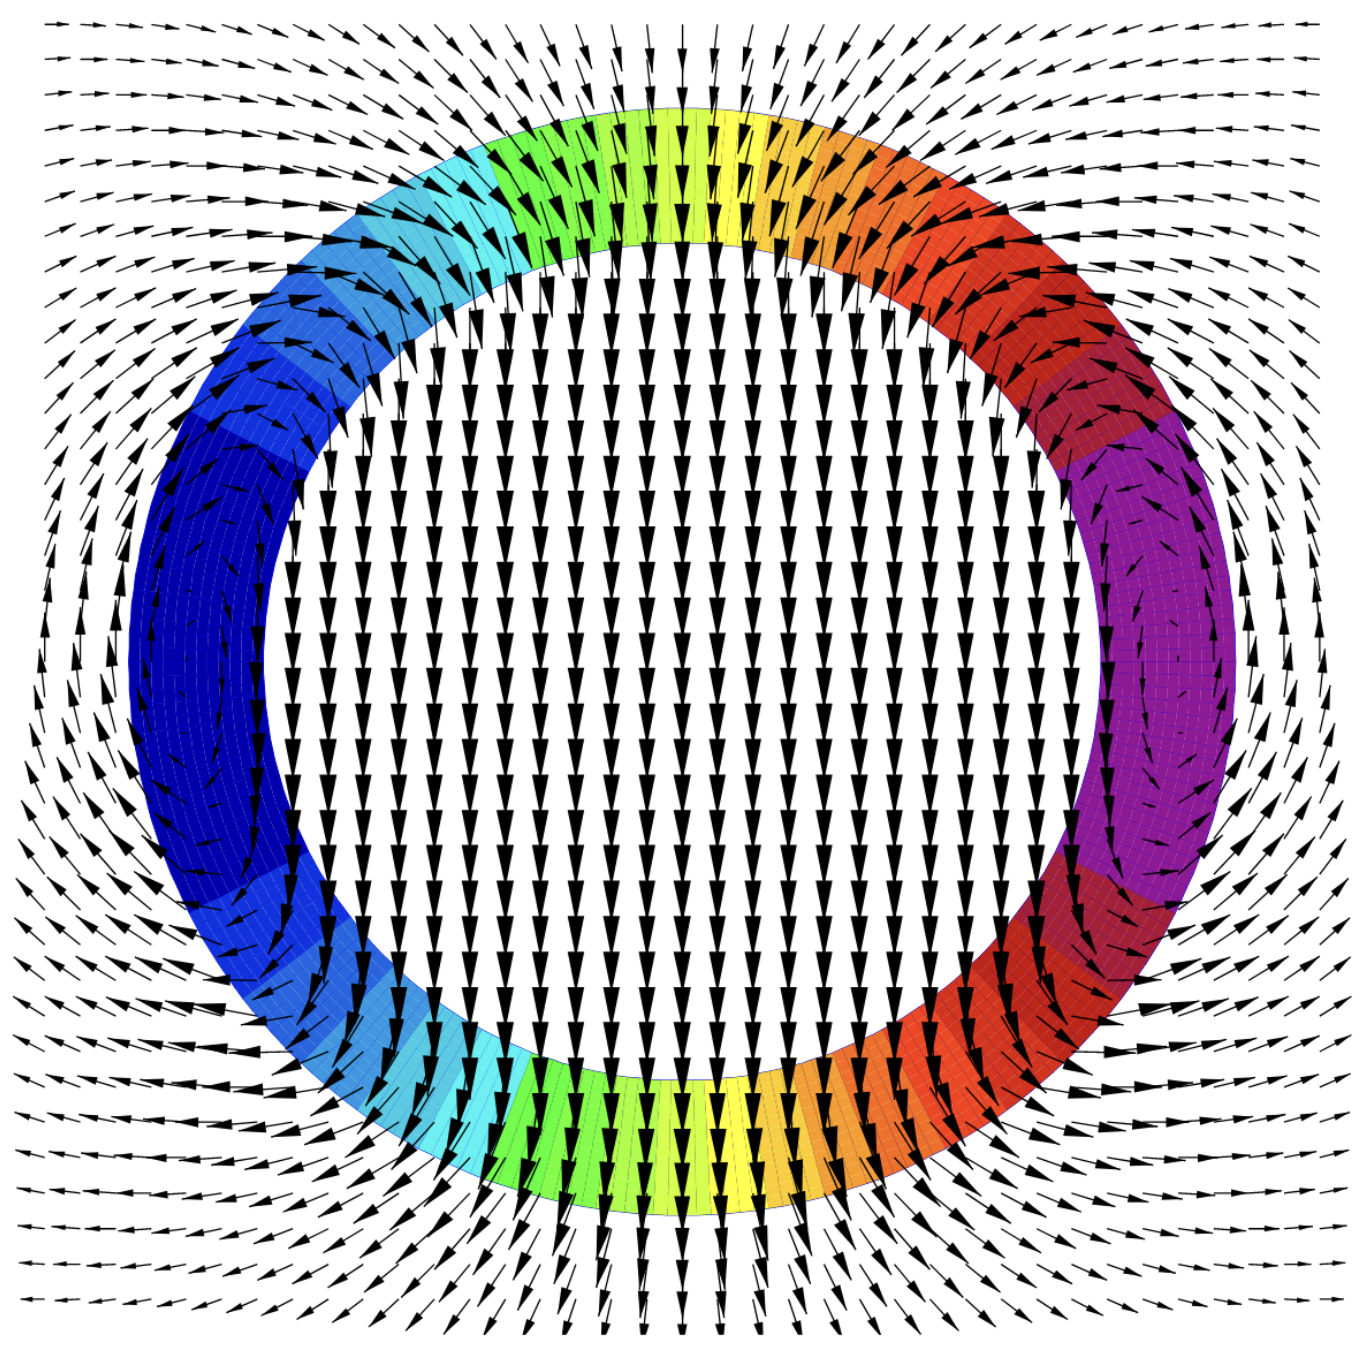
\includegraphics[width=6.5cm]{Figures/Chapter2/ideal_dipole_cos_theta.png}
        \label{fig:ideal_dipole}
    }
    \hspace{0.5cm}
    \subfloat[.7\linewidth][Ideal quadrupole.]{
        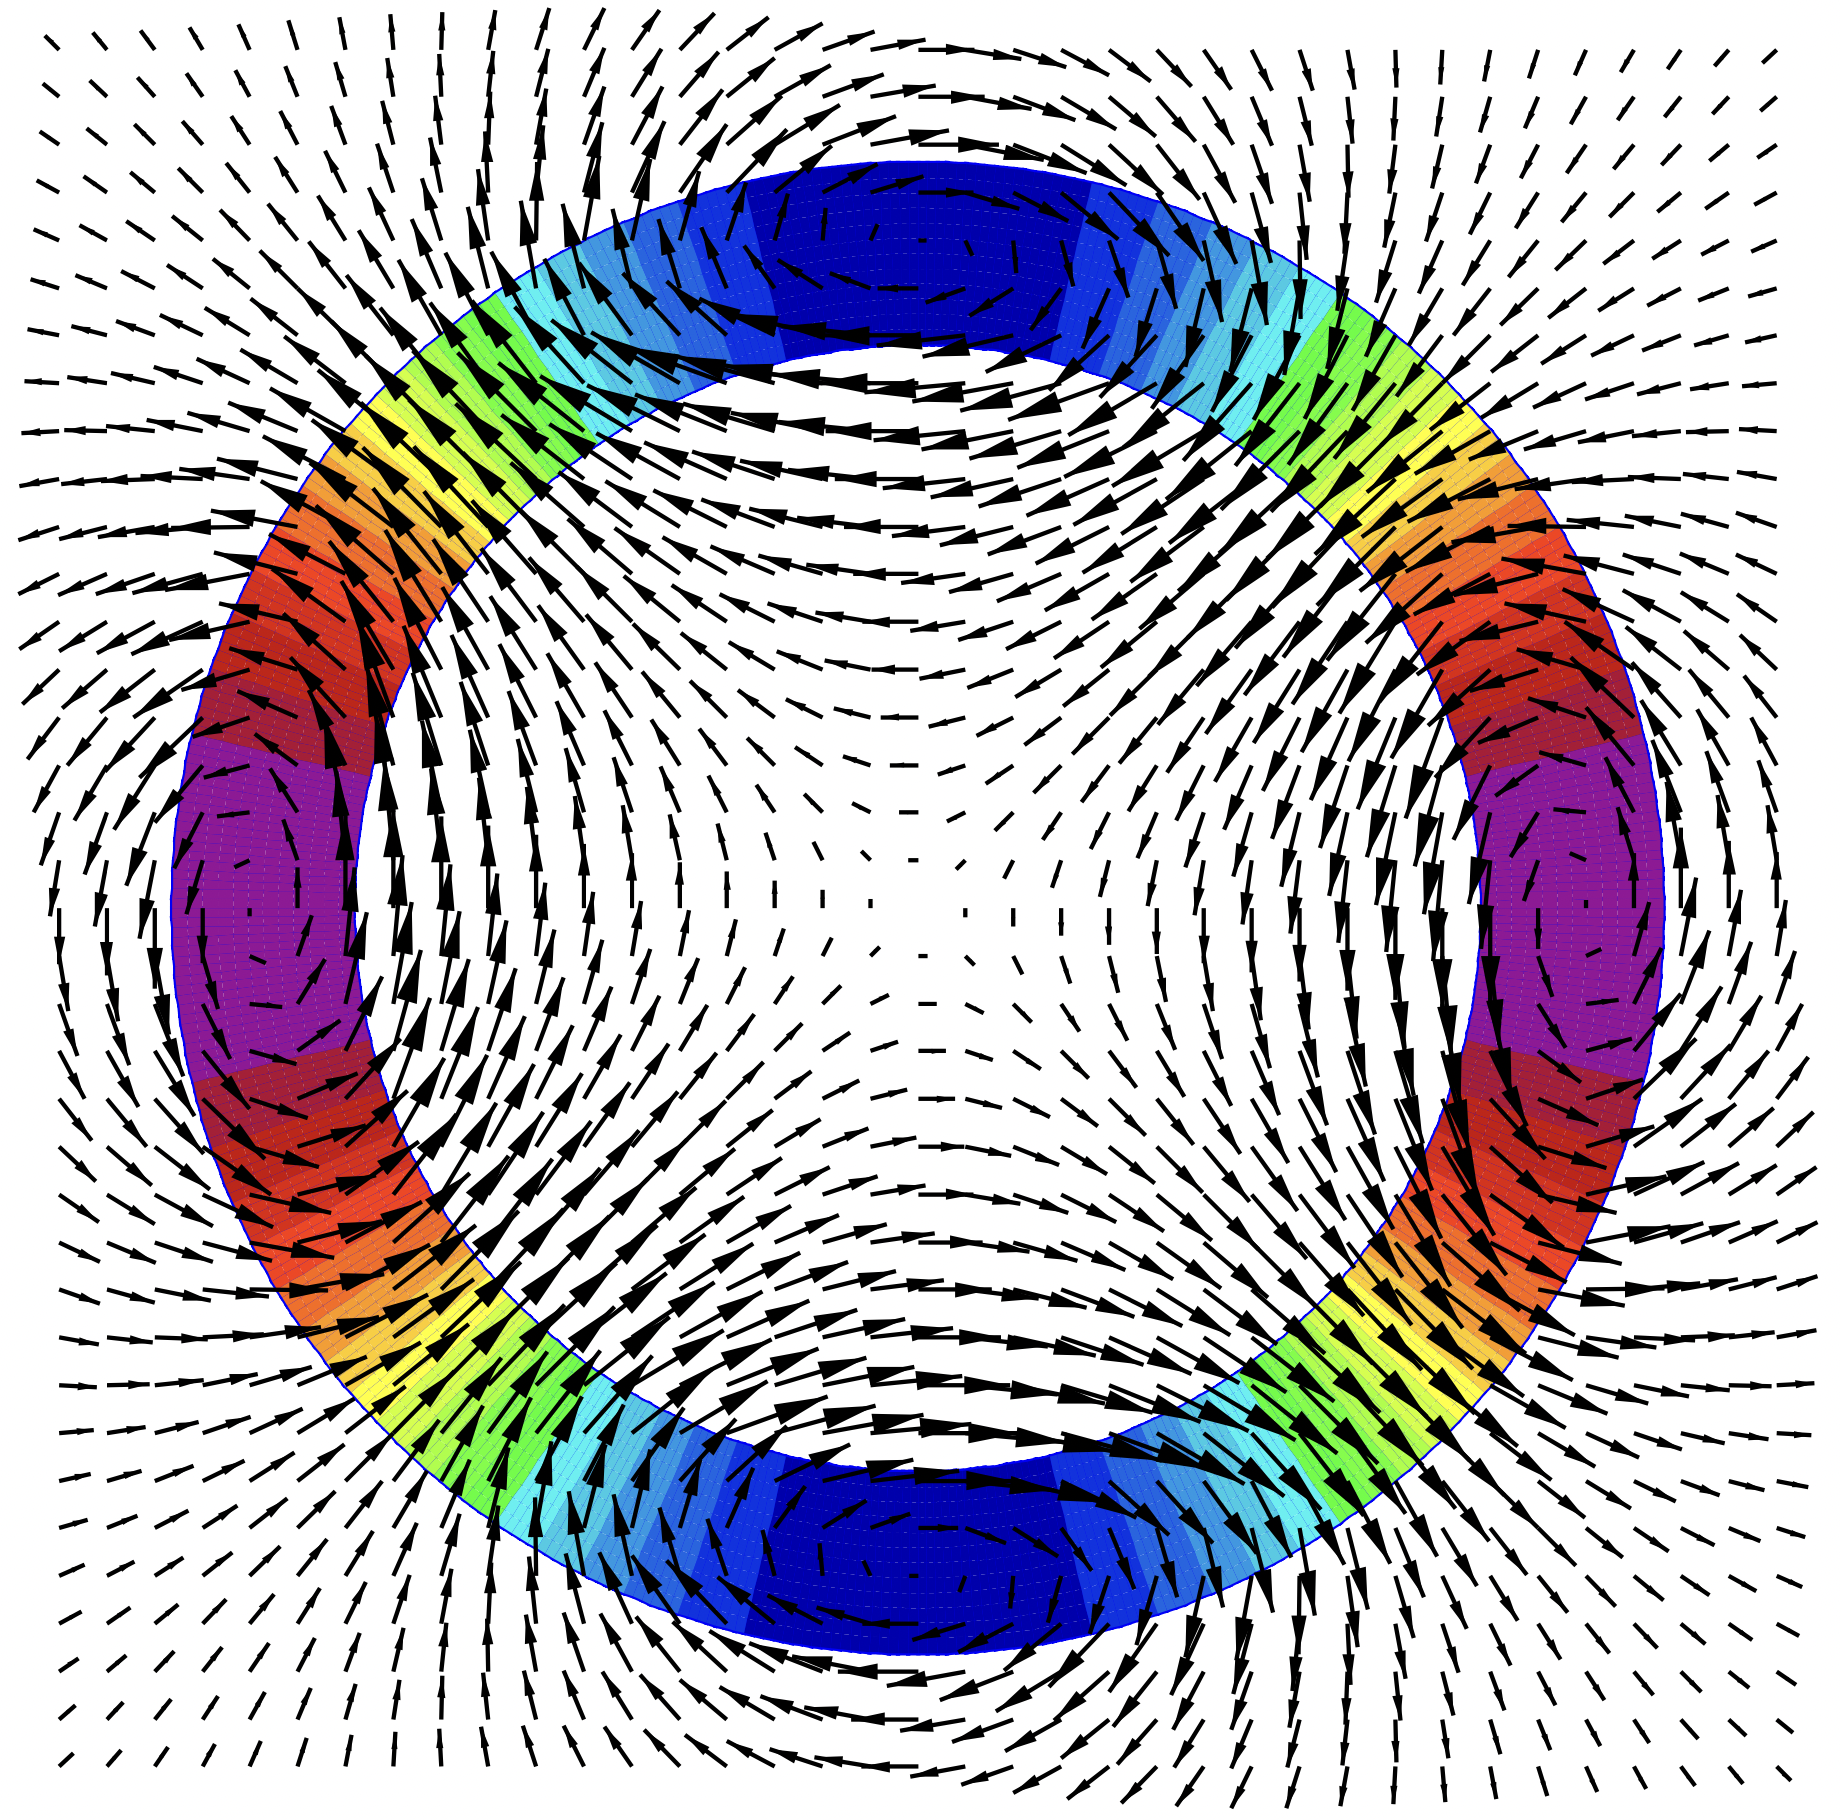
\includegraphics[width=6.5cm]{Figures/Chapter2/ideal_quadrupole_cos_2theta.png}
        \label{fig:ideal_quadrupole}
    }
    \caption{Magnetic fields and forces in an idealized dipole and quadrupole, with a \(\cos(\theta)\) and \(\cos(2\theta)\) current distribution in the circular coil, respectively. Current in the dipole and quadrupole coils are indicated in color. These visuals were taken from \cite{CERN:Russenschuck:CAS_Design_Magnets}.}
    \label{figure:dipole_quadrupole_fields}
\end{figure}

\subsection{Equations of Motion and Twiss Parameters}

The focusing from quadrupoles in a circular accelerator such as the LHC is periodic in \(s\), with a period of at most the circumference of the machine.
Assuming the existence of a closed orbit, the transverse motion of a single particle in a synchrotron with a periodic lattice is described by Hill's equation:

\begin{equation}
    u^{\prime \prime} + K_u(s) u(s) = 0; \quad u = x, y; \quad u^{\prime} = \dfrac{du}{ds} \text{ ,}
    \label{equation:hill_equation}
\end{equation}

where \(k\) describes the focusing forces action on the beam, and varies with \(s\) as it is dictated by magnetic elements traversed by particles.
A focusing quadrupole has a \(k > 0\), a focusing quadrupole has \(k < 0\), and a drift space has \(k = 0\).
The focusing strengths in the transverse planes go as:

\begin{equation}
	\begin{aligned}
		K_{x} &= \frac{1}{\rho^2} - k_{1} \text{ ,} \\
    	K_{y} &= k_{1} \text{ .}
	\end{aligned}
    \label{equation:transverse_focusing_strengths}
\end{equation}

The term \(\left(1 / \rho^2\right)\) in the horizontal component arises from the weak focusing caused by dipoles.
In the material below, \(u\) will be used to denote either \(x\) or \(y\), the rules applying to both similarly.
According to the theorem of Floquet~\cite{BOOK:Lee:Accelerator_physics}, the solution with periodic boundary conditions to Hill’s equation takes the form of \cref{equation:hill_solution}:

\begin{equation}
    \begin{aligned}
        u(s)          &= \sqrt{\beta_{u}(s) \varepsilon_{u}} \cos \left( \phi_{u}(s) + \phi_{u,0} \right) \text{ ,} \\
        u^{\prime}(s) &= -\sqrt{\frac{\varepsilon_u}{\beta_u(s)}} \left( \sin \left(\phi_u(s) + \phi_{u, 0} \right) + \alpha(s) \cos \left( \phi_u(s)+\phi_{u, 0} \right) \right) \text{ .}
    \end{aligned}
    \label{equation:hill_solution}
\end{equation}

These equations describe a harmonic oscillation in the transverse planes.
Here \(\varepsilon_u\) is the \intro{geometric emittance} of a particle and is a constant of the motion at a given energy. 
\(\phi_u(s)\) is the \intro{phase advance} and \(\alpha_u(s)\) is the \intro{alpha-function}.
\(\beta_u(s)\) is the \intro{beta-function} and represents the fluctuation of the oscillation envelope around the ring: it describes the transverse position dependent amplitude of the oscillation and has the dimension of a length.
In particle colliders such as the LHC the \betafunctions at the Interaction Points (IP), where the beams are made to collide, are commonly referred to as \(\beta_u^{\ast}\).
The solution of Hill's equation can also be written in matrix form as:

\begin{equation}
    \left(
        \begin{array}{c}
            u(s) \\
            u^{\prime}(s)
        \end{array} \right) = \mathrm{M} \left( 
        \begin{array}{c}
            u(0) \\
            u^{\prime}(0)
    \end{array} \right) \text{ ,}
    \label{equation:hill_solution_matrix}
\end{equation}

In this form, which makes the assumption that the magnetic field of an element is constant along the longitudinal direction, M is called a \intro{transfer matrix}. 
Below are the transfer matrices corresponding to a drift space, \(\mathrm{M_{drift}}\), a dipole, \(\mathrm{M_{dip.}}\), a focusing quadrupole, \(\mathrm{M_{foc. quad.}}\), and a defocusing quadrupole \(\mathrm{M_{defoc. quad.}}\), respectively.

\begin{equation}
    \mathrm{M_{drift}} = \left(
        \begin{array}{ll}
            1 & L \\
            0 & 1
    \end{array} \right) \text{ ,}
    \label{equation:drift_transfer_matrix}
\end{equation}

\begin{equation}
    \mathrm{M_{dip.}} = \left(
        \begin{array}{cc}
            \cos \theta           & \rho \sin \theta \\
            - \sin \theta / \rho  & \cos \theta
    \end{array} \right) \text{ ,}
    \label{equation:dipole_transfer_matrix}
\end{equation}

\begin{equation}
    \mathrm{M_{foc. quad.}} = \left(
        \begin{array}{cc}
            \cos \left( \sqrt{k_1} L \right)             & \frac{1}{\sqrt{k_1}} \sin \left( \sqrt{k_1} L \right) \\
            -\sqrt{k_1} \sin \left( \sqrt{k_1} L \right) & \cos \left( \sqrt{k_1} L \right)
    \end{array} \right) \text{ ,}
    \label{equation:focusing_quad_transfer_matrix}
\end{equation}

\begin{equation}
    \mathrm{M_{defoc. quad.}} = \left(
        \begin{array}{cc}
            \cosh \left( \sqrt{\abs{k_1}} L \right)                 & \frac{1}{\sqrt{\abs{k_1}}} \sinh \left( \sqrt{\abs{k_1}} L \right) \\
            \sqrt{\abs{k_1}} \sinh \left( \sqrt{\abs{k_1} L} \right) & \cosh \left( \sqrt{\abs{k_1}} L \right)
    \end{array} \right) \text{ ,}
    \label{equation:defocusing_quad_transfer_matrix}
\end{equation}
where \(L\) is the element length and \(\theta = L / \rho\) is the bending angle of the dipole.
The transfer matrix of a group of elements is obtained by multiplying the transfer matrices of all individual elements.
For example, the transfer matrix corresponding to the \(\mathrm{FODO}\) cell of \cref{figure:fodo_cell_schematic} is:

\begin{equation}
    \mathrm{M_{FODO}} = \mathrm{M_{foc. quad.}} \mathrm{M_{drift}} \mathrm{M_{defoc. quad.}} \mathrm{M_{drift}} \text{ .}
    \label{equation:fodo_transfer_matrix}
\end{equation}

For a complete machine with hundreds to thousands of elements, the maps of linear elements can still be combined to obtain the coordinates of a particle after a full revolution.
This specific transfer map is called the \intro{one-turn map} and fully describes the linear evolution of a particle's coordinates over one revolution of the accelerator.
It can be expressed as

\begin{equation}
    \mathrm{M_{OTM}} = \mathrm{M_N} \cdot \mathrm{M_{N-1}} \cdot \ldots \cdot \mathrm{M_2} \cdot \mathrm{M_1} \text{ ,}
    \label{equation:one_turn_map}
\end{equation}
where \(\mathrm{M_i}\) is the transfer matrix of the \(i\)th element in the machine.
The transformation of coordinates over a revolution is then given by

\begin{equation}
    \left(
        \begin{array}{c}
            u \\
            u^{\prime}
        \end{array} \right)_{s_0 + C} = \mathrm{M_{OTM}} \cdot \left( 
        \begin{array}{c}
            u \\
            u^{\prime}
    \end{array} \right)_{s_0} \text{ .}
    \label{equation:one_turn_coordinates_transformation}
\end{equation}

The phase advance \(\phi_u(s)\) mentioned above corresponds to the difference of the betatron phase functions at two points, typically also taken with respect to an arbitrary initial point at \(s = 0\).
The phase advance between two points at longitudinal positions \(s_1\) and \(s_2\) in the lattice is defined as:

\begin{equation}
    \phi_{s_1 \rightarrow s_2} = \phi(s_{2}) - \phi(s_{1}) = \int_{s_{1}}^{s_{2}} \frac{1}{\beta(s)} ds \text{ .}
\end{equation}

As particles go around the ring, they oscillate around the closed orbit within an enveloppe defined by the \betafunctions and the emittance.
The number of these so-called \intro{betatron oscillations} per revolution is the \intro{tune} \(Q_u\).
The tune is defined in \cref{equation:tune_definition}, where $\Delta \phi_{x, y}$ is the total betatron phase advance of a particle over a full circumference:

\begin{equation}
    Q_{u} = \frac{1}{2 \pi} \Delta \phi_{u} = \frac{1}{2 \pi} \oint_C \dfrac{ds}{\beta_{u} (s)} \text{ .}
    \label{equation:tune_definition}
\end{equation}

The \alphafunction is defined via the derivative of the \betafunction by:

\begin{equation}
    \alpha_u(s) = - \frac{1}{2} \beta^{\prime}_u(s) \text{ .}
    \label{equation:alpha_function}
\end{equation}

Similarly to the \(\beta\)-function, the \intro{gamma-function} $\gamma_u(s)$ describes the envelope of oscillations in \(x^{\prime}\) and \(y^{\prime}\).
Both quantities are related by the \alphafunction according to:

\begin{equation}
    \gamma_u(s) = \frac{1 + \alpha_u^2(s)}{\beta_u(s)} \text{ .}
    \label{equation:gamma_function}
\end{equation}

The \(\alpha_u (s)\), \(\beta_u (s)\), \(\gamma_u (s)\) and \(\phi_u (s)\) are also called the \intro{Twiss parameters}.
The transfer matrix can be expressed with Twiss parameters according to~\cite{AOP:COURANT:Theory_Alternating_Gradient_Synchrotron}:

\begin{equation}
    \mathrm{M} = 
    \left( 
    \begin{array}{ll}
        m_{11} & m_{12} \\
        m_{21} & m_{22}
    \end{array} \right) 
    = 
    \left(
    \begin{array}{cc}
        \cos(\phi_u) + \alpha_u \sin(\phi_u) & \beta_u \sin(\phi_u) \\
        - \gamma_u \sin(\phi_u)              & \cos(\phi_u) - \alpha_u \sin(\phi_u)
    \end{array} 
    \right) \text{ .}
    \label{equation:transfer_matrix_twiss_parameters}
\end{equation}

\subsection{Phase Space Ellipse}

In the linear regime all particle trajectories describe ellipses in \((u, u^{\prime})\) phase space.
The geometric emittance \(\varepsilon_u\) introduced in \cref{equation:hill_solution}, also named the \intro{Courant-Snyder invariant}, defines together with the Twiss parameters \(\alpha_u (s)\), \(\beta_u (s)\) and \(\gamma_u (s)\) the equation of the phase space ellispe:

\begin{equation}
    \gamma_{u}(s) u^{2} + 2 \alpha_{u}(s) u(s) u^{\prime}(s) + \beta_{u}(s) u^{\prime}(s)^{2} = \varepsilon_u \text{ .}
    \label{equation:ellipse_equation}
\end{equation}

\Cref{figure:phase_space_ellipse} shows a schematic illustration of the phase space ellipse, the area of which is defined by the geometric emittance according to:

\begin{equation}
    A = \pi \varepsilon_u \text{ .}
    \label{equation:phase_space_ellipse_area}
\end{equation}

\begin{figure}[!htb]
    \begin{center}
    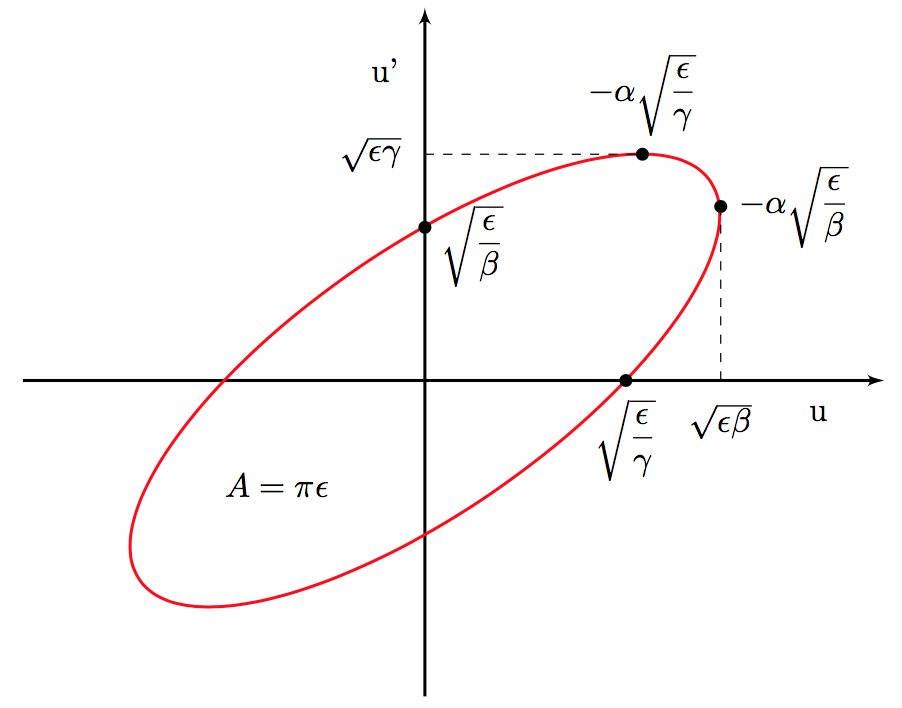
\includegraphics[width = 0.75\linewidth]{Figures/Chapter2/Phase_Space.png}
    \caption{Phase space ellipse in the transverse \((u, u^{\prime})\) plane, where \(u\) represents either transverse coordinate \(x\) or \(y\).}
    \label{figure:phase_space_ellipse}
    \end{center}
\end{figure}

According to the Liouville theorem, the phase space volume, the ellipse area \(A\) is a constant in a closed system.
When accelerating the beam this theorem no longer holds true and the geometric emittance \(\varepsilon\) will decrease as the beam energy increases.
One can then construct the \intro{normalized emittance} \(\varepsilon_{\gamma}\), which is invariant with beam energy, based on the relativistic beta and gamma:

\begin{equation}
    \varepsilon_u^{\mathrm{norm}} = \beta_{\mathrm{rel}} \gamma_{\mathrm{rel}} \varepsilon_u \text{ ,}
    \label{equation:normalized_emittance}
\end{equation}

When referring to the emittance of a specific particle one uses the term \intro{single particle emittance}.
The \intro{action} \(J_u\) is related to the single particle emittance by:

\begin{equation}
    2 J_u = \varepsilon_u \text{ .}
    \label{equation:single_particle_action}
\end{equation}

The state of particles in phase space can be fully characterized by the action variable and the corresponding phase variable seen above. 

Different particles in the beam will have different single particle emittances and will undergo betatron oscillations of varying amplitudes.
For a Gaussian shaped beam the transverse beam size is defined as:

\begin{equation}
    \sigma_u = \sqrt{\beta_u(s) \varepsilon_u^{\mathrm{beam}}} \text{ ,}
    \label{equation:gaussian_beam_transverse_beam_size}
\end{equation}
with \(\varepsilon_u^{\mathrm{beam}}\) the beam emittance, typically defined the emittance corresponding to a \(1 \sigma\) amplitude of the Gaussian charge distribution.
In the case of more general particle distributions an alternative definition of the beam emittance is often used~\cite{CERN:Muller:Beam_Matter_Covariance_Matrix_Emittance, CERN:Buon:CAS_Beam_Phase_Space_Emittance}:

\begin{equation}
    \varepsilon_u^{\mathrm{rms}} = \sqrt{\left\langle u \right\rangle^{2} \left\langle u^{\prime} \right\rangle^{2} - \left\langle uu^{\prime} \right\rangle^{2}} \text{ .}
    \label{equation:beam_emittance_general}
\end{equation}

The phase space trajectory of a particle depends on the Twiss parameters $\alpha(s)$, $\beta(s)$, and $\gamma(s)$.
One can remove this dependency by performing a coordinate transformation to the \intro{Courant-Snyder coordinates}~\cite{BOOK:Bazzani:Normal_Form_Approach_Betatron_Motion}, defined as:

\begin{equation}
    \left(\begin{array}{c}
    \hat{u} \\
    \hat{u}^{\prime}
    \end{array}\right) = \left(\begin{array}{cc}
    \frac{1}{\sqrt{\beta_{u}(s)}} & \frac{\alpha_{u}(s)}{\sqrt{\beta_{u}(s)}} \\
    0 & \sqrt{\beta_{u}(s)}
    \end{array}\right)\left(\begin{array}{c}
    u \\
    u^{\prime}
    \end{array}\right) \text{ ,}
    \label{equation:courant_snyder_coordinates}
\end{equation}
where the Courant-Snyder coordinates are denoted by \^{}.
In this new system particles follow circular trajectories in phase space.

\subsection{Chromatic Effects}

Until now, it was assumed that all particles had the intended design momentum \(p_{0}\).
Naturally, in practice particles withing the beam have a distribution in energy and momentum.
For a particle with a momentum \(p \neq p_{0}\) one defines and uses the \textit{relative momentum deviation} \(\delta\): the deviation from the reference orbit from the momentum deviation.

\begin{equation}
    \delta = \frac{p - p_{0}}{p_{0}} = \frac{\Delta p}{p} \text{ .}
    \label{equation:momentum_deviation}
\end{equation}

Such momenta offsets introduce \intro{chromatic errors} in the beam dynamics.
Effects and parameters depending on \(\delta_p\) are called \intro{chromatic effects}.

From the definition of the magnetic rigidity in \cref{equation:magnetic_rigidity}, it follows that particles of different momenta will have different local radii of curvature when going through dipoles and therefore follow different orbits along the machine.
The deviation of an off momentum particle orbit from that of the synchronous particle is defined by the \intro{dispersion function} $D(s)$.
Its contribution to a particle's orbit in a region of non-zero dispersion is described by:

\begin{equation}
    \Delta u_{\mathrm{dispersion}} = D_{u}(s) \delta 
    \label{equation:dispersion_contribution_to_orbit}
\end{equation}
\bigbreak

Off-momentum particle positions scale linearly with dispersion, and in its presence \cref{equation:hill_solution} is extended to~\cite{BOOK:Wiedemann:Particle_Accelerator_Physics}:

\begin{equation}
    u(s) = \sqrt{\varepsilon_u \beta_u(s)} \cos \left( \phi_u(s) + \phi_{u, 0} \right) + D_u(s) \delta_p
\end{equation}

Another chromatic parameter is the \intro{chromaticity} \(Q_u^{\prime}\), which describes the tune shift \(\Delta Q_u\) with particle momentum by

\begin{eqnarray}
    Q^{\prime}_u = \frac{\Delta Q_u}{\delta_p} \text{ .}
    \label{equation:chromaticity_definition}
\end{eqnarray}

The effective focusing strength of quadrupoles, which is inversely proportional to the momentum, differs for off momentum particles.
The change of focusing strength due to energy deviation is:

\begin{equation}
	\Delta k_{1} = - \dfrac{e}{p^2} \dfrac{d B_{y}}{d x} \Delta p = -k_{1} \delta_p \text{ .}
    \label{equation:quadrupole_focusing_strength_deviation_from_dispersion}
\end{equation}

This quadrupole error results in a tune shift proportional to the energy offset:

\begin{equation}
	\Delta Q = \dfrac{1}{4 \pi} \int \beta(s) \Delta k_{1}(s) ds = \left[ - \frac{1}{4 \pi} \int \beta(s) k_{1}(s) ds \right] \delta \text{ .}
    \label{equation:tune_shift_from_dispersion}
\end{equation}

The natural chromaticity of a linear lattice can then be approximated by~\cite{CAS:Guiducci:Chromaticity}:

\begin{equation}
    Q_u^{\prime} \approx -\frac{1}{4 \pi} \oint \beta_u(s) K_u \mathrm{d}s \text{ .}
    \label{equation:natural_chromaticity_approximation}
\end{equation}

%----------------------------------------------------------------------------------------

\section{Non-Linear Magnetic Multipoles}

Magnetic fields of sextupolar and higher order are called \intro{non-linear} magnetic fields.
While only dipolar and quadrupolar magnetic fields are considered in the linear approximation, non-linear magnetic fields are present in most accelerators.
They can be introduced by design or by the presence of flaws in lower order magnets, the latter having the potential to seriously disrupt the beam.

The order of a multipole is labeled \(n\), with the convention that \(n = 1\) corresponds to a magnetic dipole, \(n = 2\) to a quadrupole, \(n = 3\) a sextupole etc.
The magnetic field of a multipole of order \(n\) is given by:

\begin{equation}
    \begin{aligned}
    B_y(x, y, s) + i B_x(x, y, s) &= \sum_{n=1}^{\infty} \left[ b_n(s) + i a_n(s) \right] (x + i y)^{n-1} \text{ ,} \\
    B_n(s)                        & = \left. \frac{1}{(n - 1) !} \frac{\partial^{n - 1} B_y}{\partial x^{n - 1}} \right|_{(0,0,s)} \text{ ,} \\
    A_n(s)                        & = \left. \frac{1}{(n - 1) !} \frac{\partial^{n - 1} B_x}{\partial x^{n - 1}} \right|_{(0,0,s)} \text{ ,} 
    \end{aligned}
    \label{equation:multipole_expansion}
\end{equation}

Here \(B_n(s)\) and \(A_n(s)\) are the normal and skew multipole coefficients, respectively, where a skew magnet is rotated by \(\pi / (2 n)\) with respect to its normal counterpart.
In the linear regime, the Hamiltonian may be written as

\begin{equation}
    \mathcal{H} = \frac{1}{2} p_x^2 + \frac{1}{2} p_y^2 + \frac{1}{2} K(s) x^2 - \frac{1}{2} K(s) y^2
    \label{equation:hamiltonian_linear_lattice}
\end{equation}
where \(K(s)\) describes the variation of focusing strength around the ring.

Starting from the Hamiltonian equations

\begin{equation}
    \dfrac{d \vec{p_z}}{d t} = - \frac{\partial \mathcal{H}}{\partial \vec{z}} \quad \quad \quad \dfrac{d \vec{z}}{d t} = \frac{\partial \mathcal{H}}{\partial \vec{p_z}} \text{ ,}
    \label{equation:hamiltonian_equations}
\end{equation}
the Hamiltonian for the transverse planes for a multipole of order n is given by \cref{equation:hamiltonian_multipole_order_n}~\cite{PHD:Tomas, PHD:Franchi}:

\begin{equation}
    \mathcal{H} = \frac{q}{p} \operatorname{Re} \left[ \left( B_n +i A_n \right) \frac{(x + i y)^n}{n} \right] \text{ .}
    \label{equation:hamiltonian_multipole_order_n}
\end{equation}

If the Hamiltonian for a normal multipole of order \(n\) is labeled \(N_n\), and the Hamiltonian for a skew multipole of order \(n\) is labeled \(S_n\), then~\cite{PHD:Maclean, PHD:Persson}:

\begin{equation}
    \begin{aligned}
        N_n \propto \operatorname{Re} \left[(x + i y)^n \right] \text{ ,} \\
        S_n \propto \operatorname{Im} \left[(x + i y)^n \right] \text{ .} \\
    \end{aligned}
    \label{equation:hamiltonian_prop_normal_and_skew_multipoles}
\end{equation}

%----------------------------------------------------------------------------------------

\section{Non-Linear Formalism and Resonance Driving Terms}










\clearpage

%----------------------------------------------------------------------------------------

% \section{Phenomenology of Non-Linear Beam Dynamics}

% \subsection{Chromaticity}

% \subsection{Detuning with Amplitude}

% \subsection{Decoherence}

%----------------------------------------------------------------------------------------

% \section{Normal Form Formalism and Resonance Driving Terms}


% The derivation in this section follows the approach given in \cite{Tomas_thesis, Franchi_thesis}.
% While the non-linear dynamics can not be described with matrices, it can be described by the transfer map formalism.
% In the frame where the one turn map is represented by a pure rotation - in normal forms coordinates - it can be written as \cite{Tomas_thesis}:\\

% \begin{equation}
%     \mathcal{M} = 
%     e^{:\eqnmarkbox[blue]{node1}{\tilde{h_{1}}}:}
%     e^{:\eqnmarkbox[red]{node2}{\tilde{h_{2}}}:}
%     \ldots
%     e^{:\eqnmarkbox[green]{noden}{\tilde{h_{n}}}:}
%     R
%     \label{equation:norm_form_one_turn_map}
% \end{equation}
% \annotate[yshift=0.5em]{above, left}{node1}{First element}
% \annotate[yshift=-0.75em]{below}{node2}{Second element}
% \annotate[yshift=0.5em]{above, right}{noden}{Nth element}\\\\
% % ------------------ %
% where \(e^{:\tilde{h_{1}}:}\) is an exponential Lie operator describing a nonlinear element, and \(\mathbf{R}\) is the rotation matrix describing the linear motion.
% This simplifies through the Campbell-Baker-Hausdorff theorem to:

% \begin{equation}
%     \mathcal{M} = e^{:h:} R
% \end{equation}

% In case the \(\tilde{h_{n}}\) are small, then \(h\) may be approximated by:

% \begin{equation}
%     h = \sum_{n=1}^{N} \tilde{h}_{n} + \sum_{n, m<n}^{N} \left[\tilde{h}_{m}, \tilde{h}_{n} \right] + \ldots
%     \label{equation:h_expansion}
% \end{equation}

% Using only the first order in \(\tilde{h_{n}}\), \(h\) may be expanded according to \cref{equation:h_approximation_first_order} using the action-angle variables TODO.

% \begin{equation}
%     h = \sum_{j k l m} h_{j k l m} \left(2 J_{x}\right)^{\frac{j+k}{2}} \left(2 J_{y}\right)^{\frac{l+m}{2}} e^{i \left[(j-k)\left(\phi_{x}-\phi_{x_{0}}\right) + (l-m)\left(\phi_{y}-\phi_{y_{0}}\right) \right]}
%     \label{equation:h_approximation_first_order}
% \end{equation}

% Here \(h_{j k l m}\) are Hamiltonian coefficients representing the contributions from multipoles of order \(n = j + k + l + m\).
% A multipole of order \(n\) generates terms in the Hamiltonian \(\propto x^{j+k} y^{l+m}\), where again \(n = j + k + l + m\).

% In the case of a skew quadrupole, such an element gives rise to terms in the Hamiltonian \(\propto xy\), meaning that it contributes to the Hamiltonian terms \(h_{1010}\), \(h_{1001}\), \(h_{0110}\) and \(h_{0101}\).
% The idea behind normal form coordinates is to perform a transformation from a system with amplitude and phase dependence to a simpler form.
% The simplest form is an amplitude dependent rotation, i.e. a rotation in phase space where the angle depends on the amplitude of the particle.
% An excellent approach to normal forms formalism can be found in \cite{Carlier_thesis}.

% The coordinate change is represented by a similarity transformation of the one turn map:

% \begin{equation}
%     e^{-: F:} e^{: h:} R e^{: F:}
% \end{equation}
% % ------------------ %
% where \(F\) is the generating function for the transformation.
% The formal solution to finding the generating function F is given in \cite{Forest_normal_forms} and the explicit expression is obtained in \cite{Tomas_thesis} as

% \begin{equation}
%     F = \sum_{j k l m} f_{j k l m} \left(2 I_{x}\right)^{\frac{j+k}{2}}\left(2 I_{y}\right)^{\frac{l+m}{2}} e^{i\left[(j-k)\left(\psi_{x}-\psi_{x_{0}}\right)+(l-m)\left(\psi_{y}-\psi_{y_{0}}\right)\right]}
%     \label{equation:F_generating}
% \end{equation}
% % ------------------ %
% where \(f_{jklm}\) are the resonance driving terms corresponding to the Hamiltonian terms \(h_{jklm}\) respectively.
% They can be expressed according to \cref{equation:f_rdts} \cite{Tomas_thesis, Franchi_thesis}, where \(Q_x\) and \(Q_y\) are the unperturbed tunes.

% \begin{equation}
%     f_{jklm} = \frac{h_{jklm}}{1 - e^{i 2 \pi \left[(j-k) Q_{x} + (l-m) Q_{y} \right]}}
%     \label{equation:f_rdts}
% \end{equation}
% % ------------------ %
% \Cref{equation:f_rdts} diverges when \(j, k, l, m, Q_x\) and \(Q_y\) satisfy the condition:

% \begin{equation}
%     (j-k) Q_{x} + (l-m) Q_{y} = p \quad \text{ where } p \in \mathcal{Z}
%     \label{equation:resonance_condition}
% \end{equation}
% % ------------------ %
% Hence, the \(f_{jklm}\) terms are the driving terms of the resonances \([(j-k),(l-m)]\).
% Every Hamiltonian term is associated with a resonance, which explains the term Resonance Driving Terms.
% The normalized Courant-Snyder coordinates are related to the action-angle variable as

% \begin{equation}
%     \begin{aligned}
%     z &= \sqrt{2 J_{z}} \cos (\phi_{z} - \phi_{z_{0}}) \\
%     p_{z} &= -\sqrt{2 J_{z}} \sin (\phi_{z} - \phi_{z_{0}}) \quad \text { where } z=x, y
%     \end{aligned}
%     \label{equation:courant_snyder_to_action_angle}
% \end{equation}
% % ------------------ %
% It is convenient to introduce the resonant basis h defined as

% \begin{equation}
%     \begin{aligned}
%     h_{z}^{\pm} &= z \pm i p_{z} = \sqrt{2 J_{z}} e^{\mp i \left(\phi_{z}-\phi_{z_{0}}\right)} \quad \text { where } z=x, y \\
%     \mathbf{h} &= \left( h_{x}^{+}, h_{x}^{-}, h_{y}^{+}, h_{y}^{-} \right)
%     \end{aligned}
%     \label{equation:resonant_basis_h}
% \end{equation}

% The transformation to a new set of Normal Form coordinates \(\left(\zeta_{x}^{+}, \zeta_{x}^{-}, \zeta_{y}^{+}, \zeta_{y}^{-}\right)\) is given by the operator \(e^{: -F :}\).
% This is expressed as

% \begin{equation}
%     \zeta_{z}^{\pm} = \sqrt{2 I_{z}} e^{\pm i \left(\phi_{z}+\phi_{z 0} \right)} = e^{:-F:} h_{z}^{\pm}
%     \label{equation:action_angle_to_normal_form}
% \end{equation}
% % ------------------ %
% where \(I_{z}\) is the invariant of motion in the new frame.
% The one-turn map in normal form coordinates is by construction an amplitude dependent rotation, and hence the motion in these coordinates as a function of the turn number N is given by

% \begin{equation}
%     \zeta_{z}^{-}(N) = \sqrt{2 I_{z}} e^{2 \pi \nu_{x} N + \phi z_{0}}
%     \label{equation:normal_form_by_turn}
% \end{equation}

% The inverse transformation from the new action-angle variables to the linearly normalized variable is to first order written as

% \begin{equation}
%     h_{z}^{-} = e^{: F:} \zeta_{z}^{-} \simeq \zeta_{z}^{-} + \left[F, \zeta_{z}^{-}\right]
%     \label{equation:inverse_normal_form_transform}
% \end{equation}

% and using \cref{equation:normal_form_by_turn} and \cref{equation:inverse_normal_form_transform} the normalized coordinates can be expressed in the form

% \begin{equation}
%     \begin{aligned}
%     h_{x}^{-}(N) &= \sqrt{2 I_{x}} e^{i\left(2 \pi \nu_{x} N - \psi_{x_{0}}\right)} - \\
%     & 2 i \sum_{jklm} j f_{jklm} \left(2 I_{x}\right)^{\frac{j+k-1}{2}} \left(2 I_{y}\right)^{\frac{l+m}{2}} e^{i \left[(1-j+k) \left(2 \pi \nu_{x} N-\psi_{x_{0}}\right) + (m-l) \left(2 \pi \nu_{y} N-\psi_{y_{0}}\right) \right]} \\
%     h_{y}^{-}(N) &= \sqrt{2 I_{y}} e^{i\left(2 \pi \nu_{y} N - \psi_{y_{0}}\right)} - \\
%     & 2 i \sum_{jklm} l f_{jklm} \left(2 I_{x}\right)^{\frac{j+k}{2}} \left(2 I_{y}\right)^{\frac{l+m-1}{2}} e^{i \left[(k-j) \left(2 \pi \nu_{x} N-\psi_{x_{0}}\right) + (1-l+m) \left(2 \pi \nu_{y} N-\psi_{y_{0}}\right) \right]}
%     \end{aligned}
%     \label{equation:normal_form_coordinates}
% \end{equation}




\section{Betatron Coupling}

When the betatronic motion of particles in transverse planes are independent of each other, they are said to be \intro{uncoupled}.
In particle colliders such as the LHC, this behaviour is typically desirable.
When these motions share a dependency, they are said to be \intro{coupled}, and one refers to this phenomenon as \intro{betatron coupling}, or linear coupling.
The transverse motions of particles in an accelerator may couple due to a variety of factors.
Solenoid and skew quadrupole fields are the primary sources of linear coupling.
An example of a skew quadrupole is given in \cref{figure:skew_quadrupole}.

\begin{figure}
    \begin{center}
    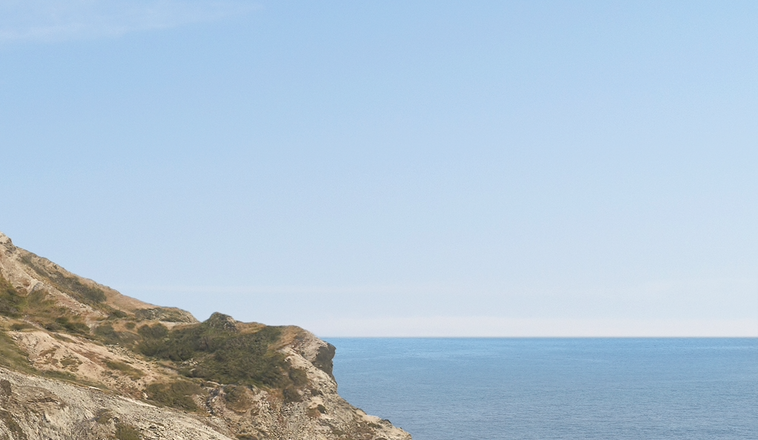
\includegraphics[width = 0.9\linewidth]{Figures/placeholder.png}
    \caption{\todo{Illustration of a skew quadrupole and its magnetic field lines.}}
    \label{figure:skew_quadrupole}
    \end{center}
\end{figure}

\subsection{Parametrization of Betatron Coupling}

\todo{Content}

\subsection{Impact and Visibility on Tunes}

Without any betatron coupling in the machine, the horizontal and vertical tunes can be matched to the same fractional value.
In the presence of betatron coupling however, the \intro{coupled fractional tunes} \(Q_1\) and \(Q_2\) cannot be matched to the same fractional value, and a minimal separation can be observed.
This separation is called the \intro{closest tune approach} and is given as the \(\Delta Q_{\mathrm{min}}\) quantity.
\Cref{figure:closest_tune_approach} shows an illustration of the phenomenon, where both the unperturbed and coupled fractional tunes are plotted against the uncoupled tune split.
The closest tune approach is the minimum distance between the two red curves, highlighted by an arrow.

\begin{figure}[!htb]
    \begin{center}
    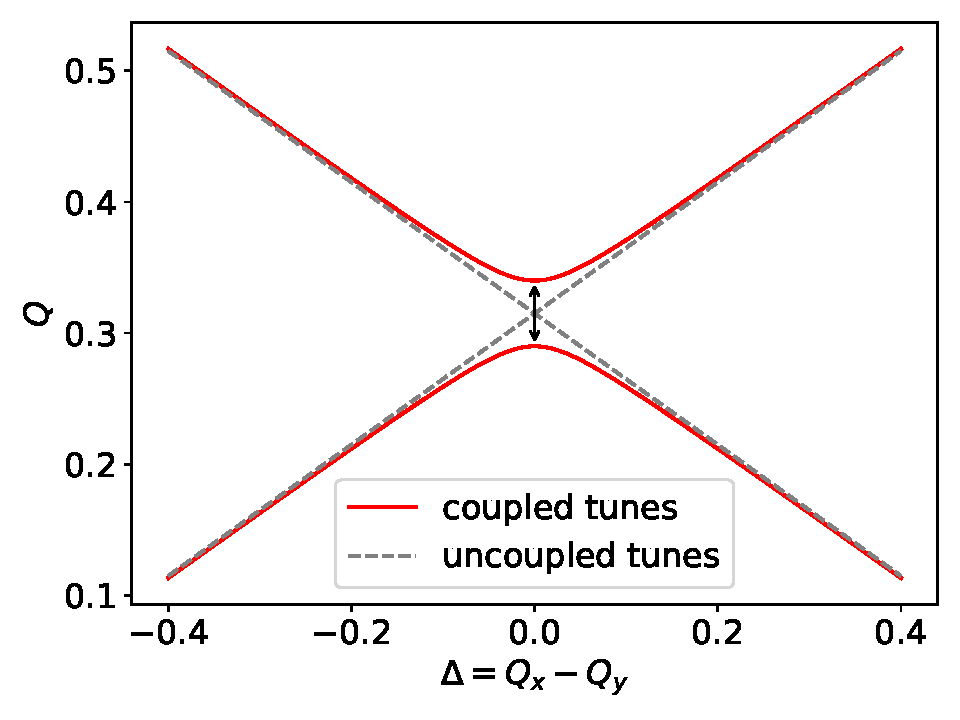
\includegraphics[width = 0.9\linewidth]{Figures/Chapter2/tune_perturbation.pdf}
    \caption{Illustration of coupled and uncoupled fractional tunes versus the uncoupled tune split.}
    \label{figure:closest_tune_approach}
    \end{center}
\end{figure}

%----------------------------------------------------------------------------------------

\section{Luminosity}

https://cds.cern.ch/record/1533084/files/CERN-THESIS-2013-022.pdf

%----------------------------------------------------------------------------------------